\documentclass[a4paper,12pt,oneside,pdflatex,italian,final,twocolumn]{article}

\usepackage[utf8]{inputenc}
\usepackage{parallel}
\usepackage{siunitx}
\usepackage{booktabs}
\usepackage{fancyhdr}
\usepackage{subcaption}
\usepackage{minted}
\usepackage{hyperref}
\usepackage{pdfpages}

\usepackage[export]{adjustbox}
\usepackage[margin=0.5in]{geometry}
\addtolength{\topmargin}{0in}

\usepackage{libertine}
\renewcommand*\familydefault{\sfdefault}  %% Only if the base font of the document is to be sans serif
\usepackage[T1]{fontenc}

\hypersetup{
	colorlinks=true, %set true if you want colored links
	linktoc=all,     %set to all if you want both sections and subsections linked
	linkcolor=blue,  %choose some color if you want links to stand out
	urlcolor=blue,   %url color
}

\definecolor{LightGray}{gray}{0.95}

\title{Custom Single Cylinder ECU}
\author{Achmadi ST MT}
\date{September 2023}

\begin{document}
	\pagestyle{fancy}
	
	\lhead{Achmadi}
	\chead{\today}
	\rhead{Specification Document}
	
	\onecolumn
	\begin{figure}
		
	\end{figure}\begin{minipage}{0.47\textwidth}
		\centering
		
	\end{minipage}
	\hfill
	\begin{minipage}{0.47\textwidth}
		\raggedleft
		\Huge \textbf{Custom Single Cylinder ECU v1}
	\end{minipage}

	\begin{figure}
		\begin{minipage}{0.47\textwidth}
			
			\section{Overview}
			\begin{itemize}
				\item Minimal and Flexible Engine Control Unit
				\item Reading TPS and RPM with calibration capability
				\item Control Injection and Ignition 
				\item Serial Data Interface in Real-time
				\item Designed to easy of use for general Injection engines
				\item Build as single circuit board with minimal setup
				\item Based on STM32Fx series that popular in automotive industries
			\end{itemize}
			
		\end{minipage}
		\hfill
		\begin{minipage}{0.47\textwidth}
			\centering
			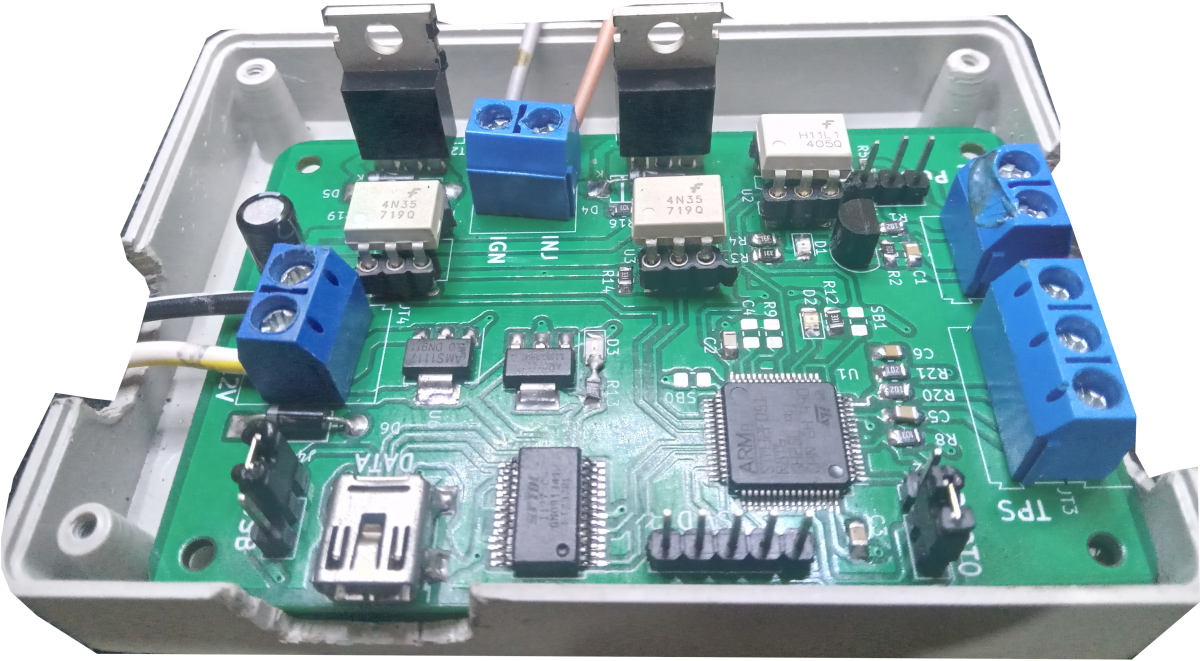
\includegraphics[width=0.8\textwidth,right]{images/unit.png}
		\end{minipage}
	\end{figure}

	\raggedright
	
	\section{Repository URLs}
	
	\begin{itemize}
		\item PCB Design: \url{https://github.com/deninur2427/ecu_pnm/tree/main/circuits/ecupnm_f051r8}
		
		\item Firmware: \url{https://github.com/deninur2427/ecu_pnm/tree/main/firmware/}
		
		\item Interface: \url{https://github.com/deninur2427/ecu_pnm/tree/main/interface/ecu_view/}
		
		\item Overall Repository: \url{https://github.com/deninur2427/ecu_pnm/}
	\end{itemize}

	\section{Technical specification}
	\centering
	\begin{tabular}{lcr}
		\toprule
		Parts & Unit & Value \\
		\midrule
		Power voltage & $V$ & 12 \\
		Main Chip & & STM32Fx LQFP64 \\
		Storage & & Internal EEPROM \\
		USB  Data Interface & & USB-Serial FT232RL \\
		Engine Control Transistor & & IRF540N \\
		TPS Input & & 12-bit ADC \\
		PULSER Input & & Any pulsed signals \\
		\bottomrule
	\end{tabular}
	
	\raggedright
	
	\newpage
	\section{Unit Preview}
	
	\begin{figure}[h]
		\centering
		\begin{subfigure}{0.45\textwidth}
			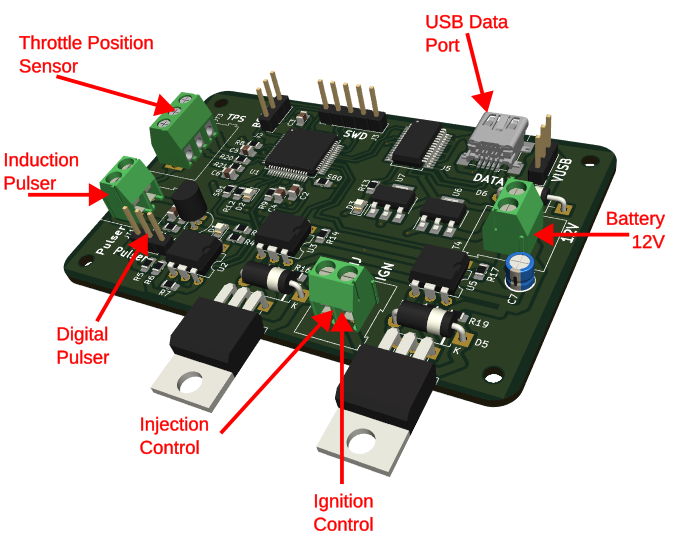
\includegraphics[width=\textwidth]{images/ecuparts.png}
			\caption{Mockup}
		\end{subfigure}
		\begin{subfigure}{0.45\textwidth}
			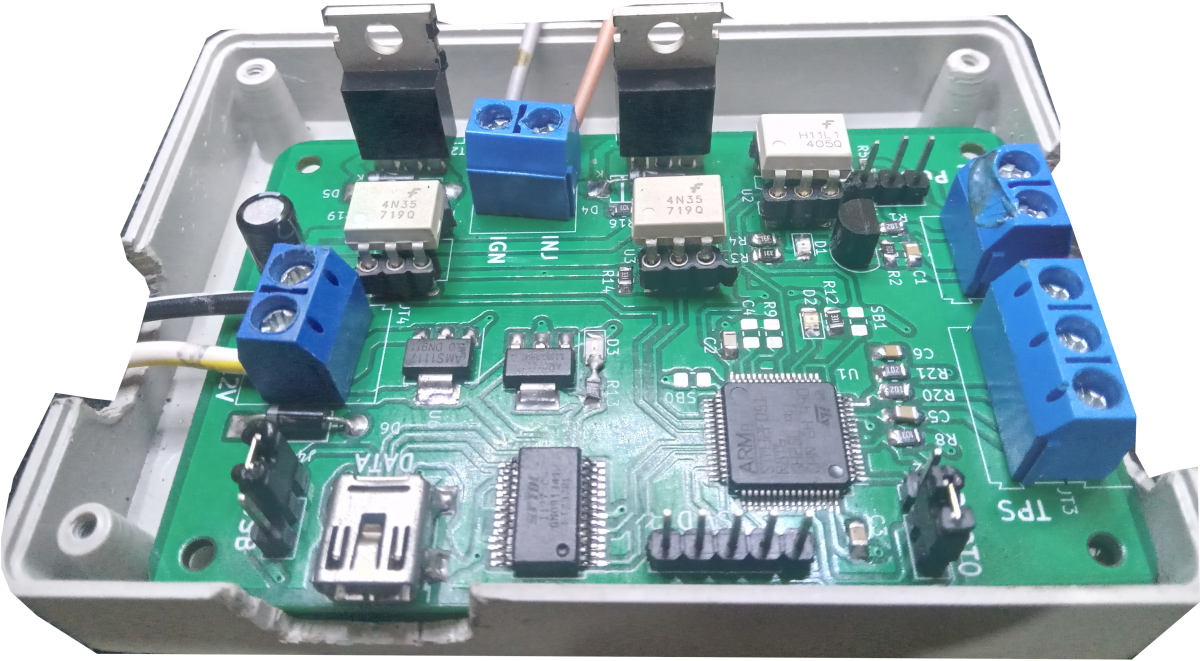
\includegraphics[width=\textwidth]{images/unit.png}
			\caption{Actual}
		\end{subfigure}
	\end{figure}

	\section{Electrical Wiring}
	
	\begin{figure}[h]
		\centering
		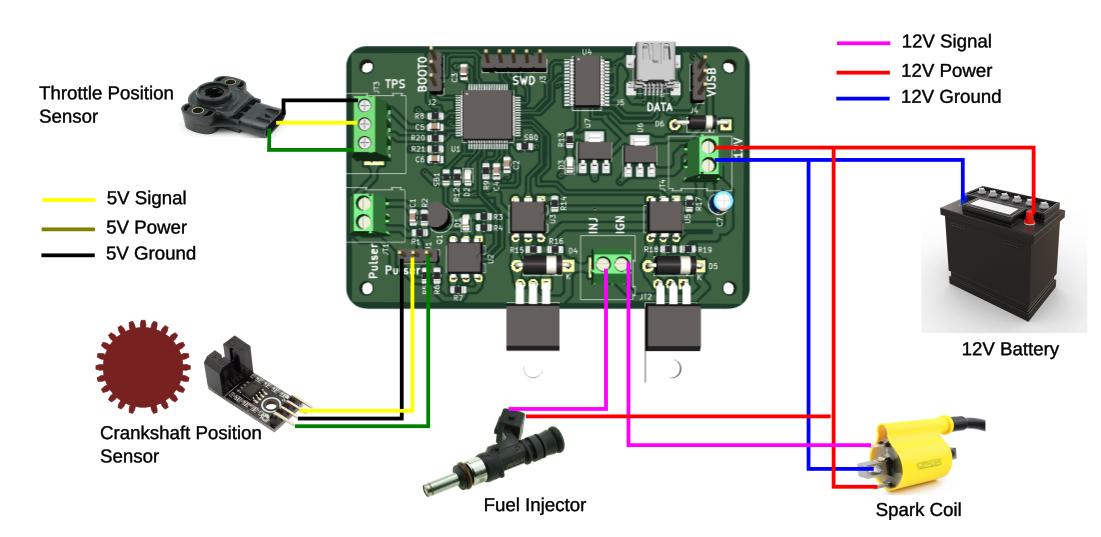
\includegraphics[width=\textwidth]{images/wiring_lqfp64.png}
		\caption{Electrical Wiring}
	\end{figure}

	\section{Schematic Design}
	
	\includepdf[pages=-,angle=-90]{images/ecupnm_sch.pdf}

	\newpage
	\section{Development Progress and Notes}
	
	List of Development Notes:
	\begin{itemize}
		\item \href{https://github.com/deninur2427/ecu_pnm/blob/main/docs/notes/tes_31072023.md}{July 31\textsuperscript{st}, 2023}
		
		\item \href{https://github.com/deninur2427/ecu_pnm/blob/main/docs/notes/tes_24082023.md}{August 24\textsuperscript{th}, 2023}
	\end{itemize}
	
\end{document}